\chapter{Results and Discussion}
\label{sec:results}

We present three different evaluations: A direct comparison between ROVIO and OKVIS on a long dataset collected indoors is shown in section \ref{sec:ijrr}, which demonstrates performance of the two algorithms and reveals drift issues. In section \ref{sec:euroc}, ROVIO results on a second complementary dataset with slower dynamics are presented, emphasizing that accuracy is dependent on the dataset. Finally, the question, if ROVIO is able to run with a generic sensor system, is approached in section \ref{sec:timesync}.

\section{Comparison of ROVIO and OKVIS on long indoor dataset}
\label{sec:ijrr}

The comparison of ROVIO and OKVIS is done on a dataset that was collected with the visual-inertial sensor unit shown in figure \ref{pics:visensor} a (Nikolic et al., \cite{nikolic2014synchronized}). The VI-sensor is equipped with two global-shutter cameras with a field of view of 120 degrees, which are hardware-wise time-synchronized to an industrial-grade ADIS 16448 IMU. There exist versions of ROVIO and OKVIS running with two or more cameras, but this work focuses on the single camera implementations, as the stereo versions do not show significantly better performance.

\begin{figure}
  \begin{subfigure}[b]{0.3\textwidth}
    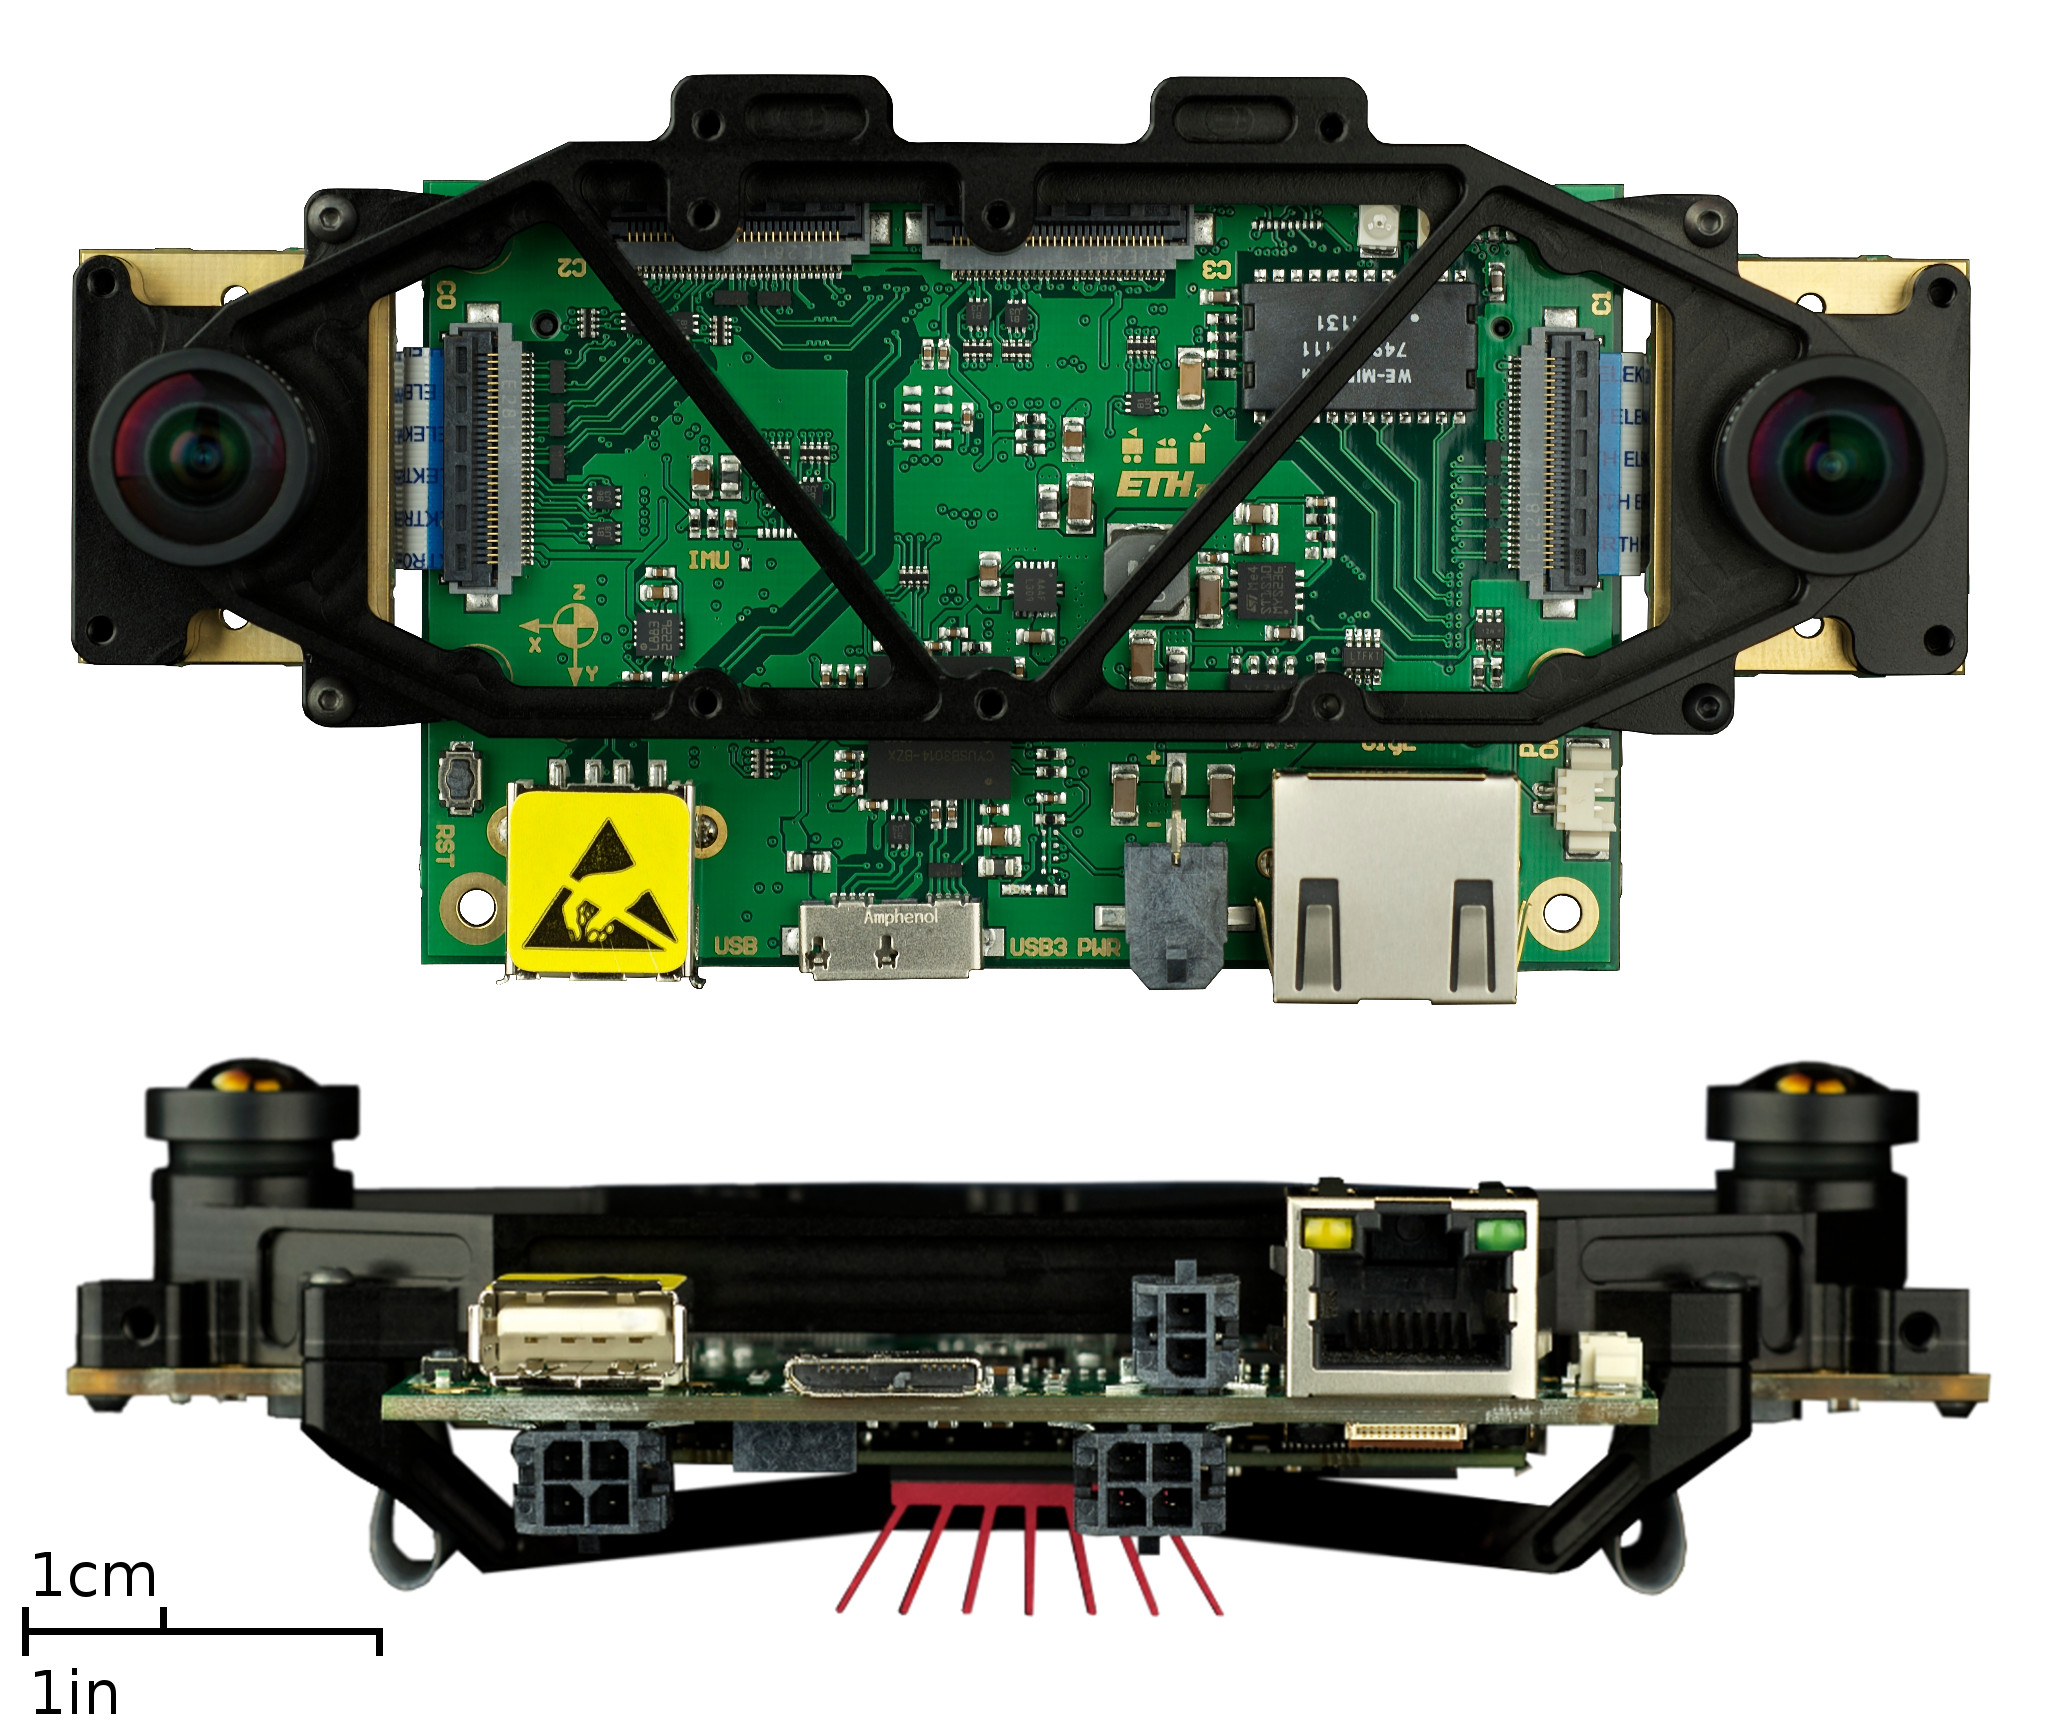
\includegraphics[width=\textwidth]{images/visensor.png}
    \caption{}
    \label{fig:1}
  \end{subfigure}
  \hfill
  \begin{subfigure}[b]{0.34\textwidth}
    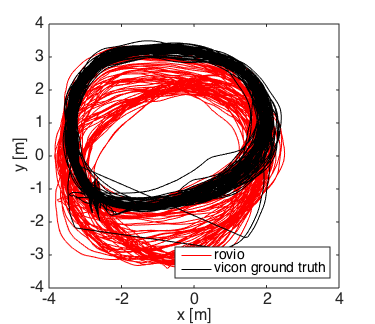
\includegraphics[width=\textwidth]{images/ijrr/2D_rovio.png}
    \caption{}
    \label{fig:2}
  \end{subfigure}
  \begin{subfigure}[b]{0.34\textwidth}
    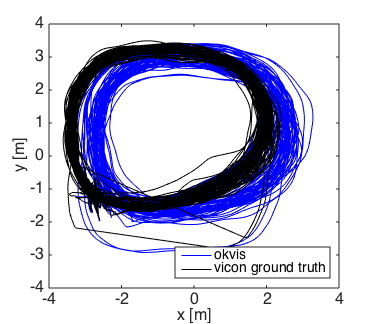
\includegraphics[width=\textwidth]{images/ijrr/2D_okvis.png}
    \caption{}
    \label{fig:2}
  \end{subfigure}
   \caption{(a) shows the visual-inertial sensor unit, equipped with two cameras and an IMU, which are hardware-wise time synchronized. (b) and (c) show the tracking performance of ROVIO and OKVIS, respectively.}
   \label{pics:visensor}
\end{figure}

The dataset has been collected by Leutenegger et al., \cite{leutenegger2015keyframe}, to demonstrate OKVIS performance. The published results on OKVIS will be compared with new results of ROVIO running on the same dataset. The data contains a trajectory with a travelled distance of 1200 $m$ collected indoors by performing approximately 100 loops within a vicon room. The camera was facing in direction of movement for the whole dataset. The camera was hand-held and moved with rather high dynamics (2 $\frac{m}{s}$ and 3 $\frac{rad}{s}$).

Figures \ref{pics:visensor} b and c show the ground truth and estimated trajectories in 2D and give a visual impression on the tracking performance of the two algorithms.

\subsection{Global accuracy}
\label{sec:ijrr_global}

Figure \ref{pics:ijrr_abs} shows the absolute translation and orientation errors of ROVIO and OKVIS for this dataset in direct comparison with median value and 25 and 75 percentiles.

After a travelled distance of 1000 $m$ ROVIO shows a translation error of 2.5 $m$ (0.25 $\%$). It is three times higher than the one of OKVIS with less than 1 $m$ ($<$0.1 $\%$). 

The absolute orientation error after a travelled distance of 1000 $m$ of ROVIO is around 45 degrees. For OKVIS it is over ten times lower with approximately 4 degrees. \\

\begin{figure}[h]
  \begin{subfigure}[b]{0.48\textwidth}
    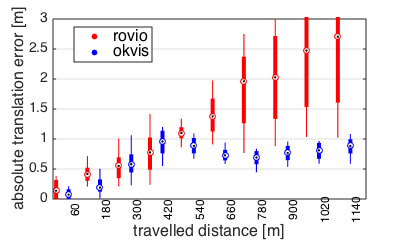
\includegraphics[width=\textwidth]{images/ijrr/ate.png}
    \caption{}
    \label{fig:2}
  \end{subfigure}
  \hfill
  \begin{subfigure}[b]{0.48\textwidth}
    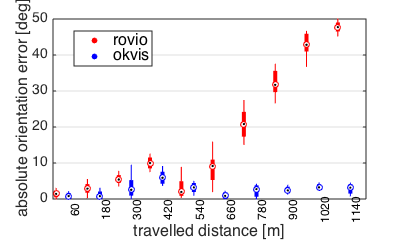
\includegraphics[width=\textwidth]{images/ijrr/aoe.png}
    \caption{}
    \label{fig:2}
  \end{subfigure}
   \caption{The absolute translation error (a) and the absolute orientation error (b) for the two algorithms in direct comparison: errors after a certain travelled distance are described with median value, 25 and 75 percentiles. After 1000 $m$, the absolute translation error of ROVIO is approximately 2.5 $m$ and 3 times higher than the one of OKVIS, the absolute orientation error is 45 degrees and 10 times higher.}
   \label{pics:ijrr_abs}
\end{figure}

To better understand what is happening over time it makes sense to look at the 6 degrees of freedom separately. Figure \ref{pics:ijrr_abs_separate} shows the errors for roll, pitch, yaw, x, y and z separately.

The roll and pitch errors (figure \ref{pics:ijrr_abs_separate} a and b) are bounded and below 1 degree for both algorithms over the whole sequence. They are 2-3 times higher for ROVIO than for OKVIS. The yaw error (figure \ref{pics:ijrr_abs_separate} c) is drifting over time, where \textit{yaw} is the orientation around the world-z axis. ROVIO shows a yaw error of 45 degrees after a travelled distance of 1000 $m$. The yaw error contains the main contribution to the absolute orientation error. Thanks to the IMU measurements, the gravity vector is observable and therefore, visual-inertial localization algorithms are only prone to drift around the world-z axis. 

The world-x and world-y errors (figure \ref{pics:ijrr_abs_separate} d and e) are mainly driven by the yaw-error and strongly dependent on the dataset itself. For a trajectory including 1000 $m$ collected in a straight line, a yaw-error of 45 degrees would sum up to large world-x and world-y errors. The world-z error (figure \ref{pics:ijrr_abs_separate} f) of ROVIO is 1 $m$ after a travelled distance of 1000 $m$, which is 3 times higher than the one of OKVIS. \\

\begin{figure}[h]
  \begin{subfigure}[b]{0.48\textwidth}
    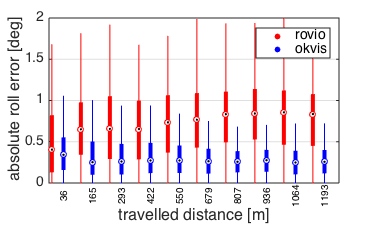
\includegraphics[width=\textwidth]{images/ijrr/aoe_r.png}
    \caption{}
  \end{subfigure}
  \hfill
  \begin{subfigure}[b]{0.48\textwidth}
    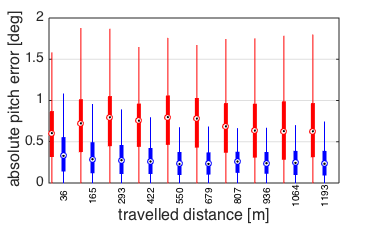
\includegraphics[width=\textwidth]{images/ijrr/aoe_p.png}
    \caption{}
  \end{subfigure}
  \begin{subfigure}[b]{0.48\textwidth}
    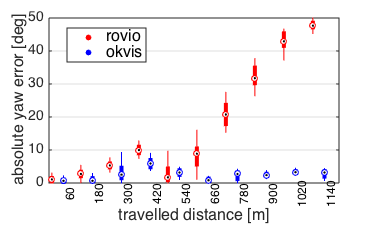
\includegraphics[width=\textwidth]{images/ijrr/aoe_y.png}
    \caption{}
  \end{subfigure}
  \hfill
  \begin{subfigure}[b]{0.48\textwidth}
    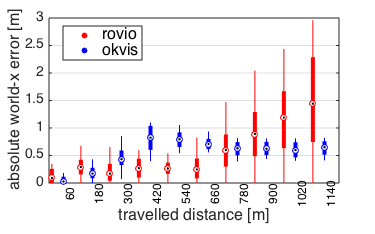
\includegraphics[width=\textwidth]{images/ijrr/ate_x.png}
    \caption{}
  \end{subfigure}
  \begin{subfigure}[b]{0.48\textwidth}
    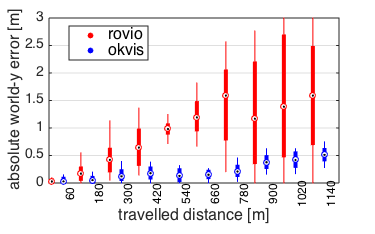
\includegraphics[width=\textwidth]{images/ijrr/ate_y.png}
    \caption{}
  \end{subfigure}
  \hfill
  \begin{subfigure}[b]{0.48\textwidth}
    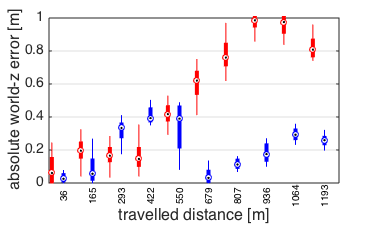
\includegraphics[width=\textwidth]{images/ijrr/ate_z.png}
    \caption{}
  \end{subfigure}
   \caption{The absolute errors for the separated axes: roll (a) and pitch (b) stay bounded and below 1 degree for both algorithms over the whole sequence. Yaw (c) is drifting over time and has the main contribution to the absolute orientation error. The world-x (d) and world-y (e) errors are mainly driven by yaw and strongly dependent on the data. The world-z error (f) of OKVIS after 1000 $m$ is three times lower than the one of ROVIO.}
   \label{pics:ijrr_abs_separate}
\end{figure}

Main results out of this analysis are: 1) OKVIS shows superior performance regarding global accuracy than ROVIO, and 2) ROVIO is prone to drift, especially in yaw, with a yaw-error of 45 degrees after 1000 $m$ of travelled distance.

The main reasons for the superior performance of OKVIS are linearization errors within ROVIO and the filtering-based property of not correcting a past estimate based on a new observation (see section \ref{sec:rovio}). 
A future way of approaching the drift issue could be to perform a global optimization in a secondary module, which takes the output of the algorithm and performs a computationally more expensive optimization on a slower rate and feeds its result back. This secondary module could also detect loop closures and increase the global accuracy significantly. Another easier way of reducing the drift issue would be to include additional sensor information of a magnetometer or even GPS into the estimation. Using only a magnetometer would make yaw observable and could decrease the yaw-drift significantly.


\subsection{Local accuracy}
\label{sec:ijrr_local}

Over short distances, the difference between the two algorithms is very small. Figure \ref{pics:ijrr_rel} shows the relative translation and orientation errors for the long indoor trajectory. The relative translation error of ROVIO is a bit higher than the one of OKVIS but in the same order of magnitude: after a travelled distance of 1 $m$, both algorithms have a median relative translation error of approximately 2 $cm$ (2 $\%$). The relative orientation error is very similar and approximately 0.6 degrees after a travelled distance of 1 $m$. \\

\begin{figure}[h]
  \begin{subfigure}[b]{0.48\textwidth}
    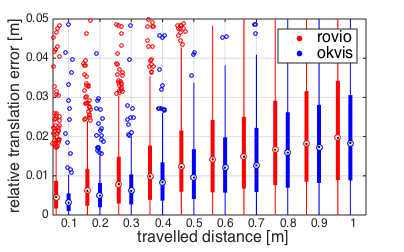
\includegraphics[width=\textwidth]{images/ijrr/rte.png}
    \caption{}
    \label{fig:2}
  \end{subfigure}
  \hfill
  \begin{subfigure}[b]{0.48\textwidth}
    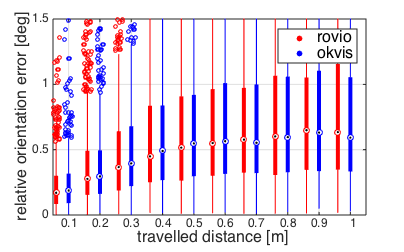
\includegraphics[width=\textwidth]{images/ijrr/roe.png}
    \caption{}
    \label{fig:2}
  \end{subfigure}
   \caption{The relative translation error (a) and the relative orientation error (b) over the travelled distance for the ROVIO and OKVIS in direct comparison: for both algorithms, the relative translation error is approximately 2 $cm$ after a travelled distance of 1 $m$. The absolute orientation error is approximately 0.6 degrees after 1 $m$ for both algorithms. The small dots on top of the figures denote outliers.}
   \label{pics:ijrr_rel}
\end{figure}

The presented results on local accuracy are hard to compare with the literature because such in depth analyses of local errors have never been published on other promising visual-inertial localization implementations. The accuracy is in a order of magnitude, which allow subsequent algorithms like dense reconstruction or object recognition to work reasonably. For direct manipulation tasks, the accuracies are probably too bad and a subsequent estimation technique for relative pose estimation between the robot and a target needs to be added.


\subsection{Computational complexity}
\label{sec:ijrr_complexity}

As mentioned in sections \ref{sec:rovio} and \ref{sec:okvis}, ROVIO and OKVIS differ in their estimation techniques and OKVIS is working with more information than ROVIO. Parts of the algorithms like the data acquisition or feature extraction are in the same order of computational complexity for the two algorithms. But the estimation itself of OKVIS is clearly more demanding. We have not been able to run OKVIS on the same machine as ROVIO and therefore, a direct comparison of computational complexity can not been demonstrated within this report. Working with a maximum number of 25 features, the processing time per frame of ROVIO on a 2.5GHz Intel Core macbook was 10 $ms$ per frame, which is rather lightweight. We know OKVIS being computationally more demanding, but still able to run in real-time on a standard laptop processor.


\section{Evaluation of ROVIO on complementary indoor dataset}
\label{sec:euroc}

The presented results have been derived on one specific dataset. To get a better impression for the presented numbers, this section will show ROVIO results on a second dataset with other characteristics, Burri et al., \cite{burri2015euroc}. It has also been collected with the VI-sensor (figure \ref{pics:visensor} a) and contains a short indoor trajectory with a travelled distance of 60 $m$. The dynamics on this dataset are slower with 1 $\frac{m}{s}$ and less than 1 $\frac{rad}{s}$. The camera was moved in direction of all body axes, not only in the direction of the optical axis and the data looks like a slowly performed random walk, see figure \ref{pics:euroc} a. \\

\begin{figure}[h]
  \begin{subfigure}[b]{0.45\textwidth}
    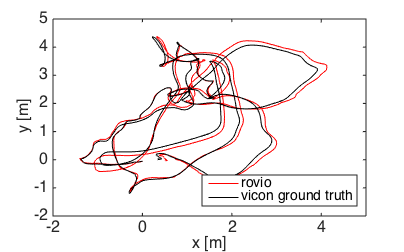
\includegraphics[width=\textwidth]{images/euroc/2D.png}
    \caption{}
  \end{subfigure}
  \hfill
  \begin{subfigure}[b]{0.45\textwidth}
    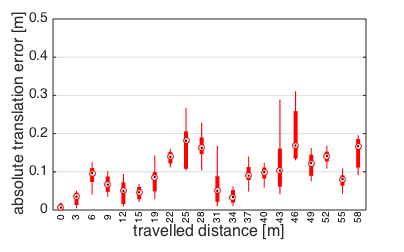
\includegraphics[width=\textwidth]{images/euroc/ate.png}
    \caption{}
  \end{subfigure}
  \begin{subfigure}[b]{0.45\textwidth}
    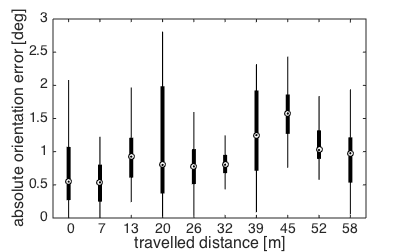
\includegraphics[width=\textwidth]{images/euroc/aoe.png}
    \caption{}
  \end{subfigure}
  \hfill
  \begin{subfigure}[b]{0.45\textwidth}
    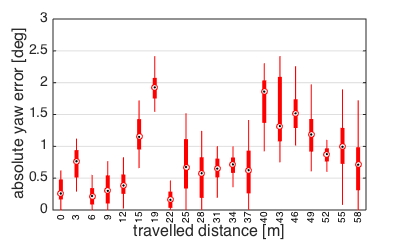
\includegraphics[width=\textwidth]{images/euroc/aoe_y.png}
    \caption{}
  \end{subfigure}
  \begin{subfigure}[b]{0.45\textwidth}
    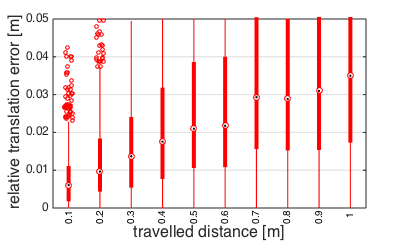
\includegraphics[width=\textwidth]{images/euroc/rte.png}
    \caption{}
  \end{subfigure}
  \hfill
  \begin{subfigure}[b]{0.45\textwidth}
    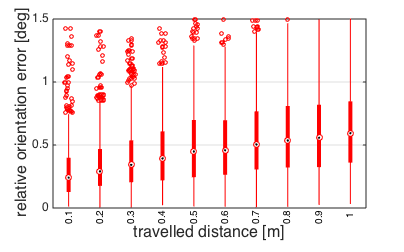
\includegraphics[width=\textwidth]{images/euroc/roe.png}
    \caption{}
  \end{subfigure}
   \caption{ROVIO performance on second dataset: the absolute translation error (b) lies between 10 $cm$ and 20 $cm$ after 50 $m$ of travelled distance and the absolute orientation error (c) after 50 $m$ is around 1 degree. The major contribution to the absolute orientation error is coming from the absolute yaw error (d). The local translation error (e) with 3-4 $cm$ after 1 $m$ is higher for this dataset than for the long trajectory and the local orientation error (f) with 0.6 degrees after 1 $m$ is similar to the long trajectory.}
   \label{pics:euroc}
\end{figure}

Looking at the global accuracy (figure \ref{pics:euroc} b, c and d) with an absolute translation error of 10-20 $cm$ and $1$ degree after a travelled distance of 50 $m$, we notice that the observed drift issues in section \ref{sec:ijrr} are not obviously visible over these short distances. Especially in yaw we can not register clear drift on this short sequence. \\

Regarding local accuracy (figure \ref{pics:euroc} e and f) a relative translation error of 3-4 $cm$ after 1 $m$ of travelled distance can be observed. This is significantly higher compared with 2 $cm$ for the long trajectory. The relative orientation error of 0.6 degrees is similar to the one of the long trajectory. The better results for the long trajectory are probably caused by the higher dynamics within that set: the IMU measurements are less noisy for higher excitements and two frames with a travelled distance of 1 $m$ in between have been captured nearer in time. \\

For a task like dense reconstruction or maintenance, this second dataset is more representative than the long trajectory, as a robot won't move with high speeds during this kind of operation. Therefore relative errors of 3-4 $cm$ and 0.6 degrees have to be expected for a travelled distance of 1 $m$.

\section{Towards a non time synchronized sensor system}
\label{sec:timesync}

All the presented results have been derived on data collected with the VI-sensor (figure \ref{pics:visensor} a). The VI-sensor is hardware-wise time synchronized, which means that the camera image capture is triggered by the IMU. Thanks to this time synchronization, the data of both sensors arrives on the visual-inertial localization algorithm accurately time-aligned. For many applications it is an important question, if a visual-inertial localization algorithm is also able to run with a more generic sensor system that does not perform a hardware time synchronization. \\

Within the scope of this report, two evaluations will be presented towards the question, if ROVIO is able to run with a sensor system, which is not hardware-wise time synchronized. In section \ref{sec:timesync_artificial}, data of the VI-sensor is passed to ROVIO, artificially modified with an added bias on the IMU timestamp. Section \ref{sec:timesync_real} shows experimental results by comparing ROVIO running on a time synchronized and on a non time synchronized sensor system.


\subsection{Artificial bias on IMU timestamp}
\label{sec:timesync_artificial}

By adding an artificial bias to the IMU timestamp, ROVIO has to deal with an inaccuracy, which is not modelled in the filter assumptions. Like that, performance decreases and the filter diverges when the bias gets too large. To get an impression, how robustly the system behaves under errors in the timestamps, hardware-wise time synchronized VI-sensor data was taken and an artificial bias on the IMU timestamp was added. \\

\begin{figure}[h]
  \begin{subfigure}[b]{0.48\textwidth}
    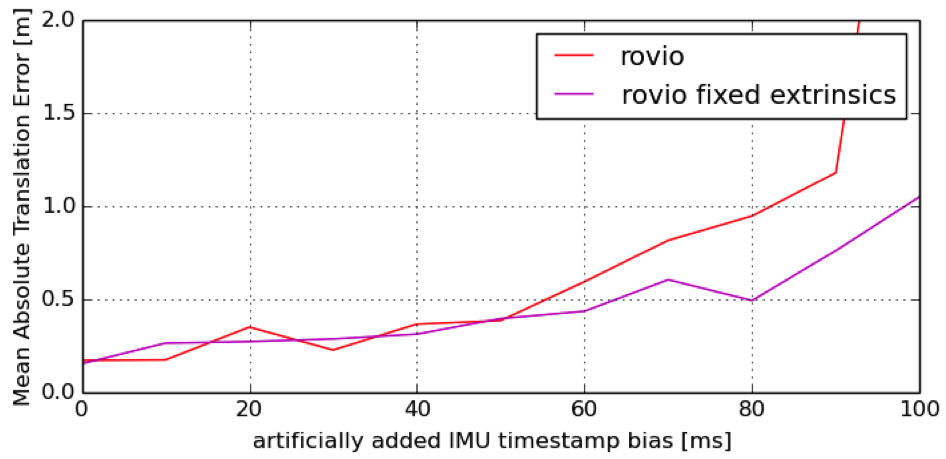
\includegraphics[width=\textwidth]{images/artificial_bias_1.png}
    \caption{}
  \end{subfigure}
  \hfill
  \begin{subfigure}[b]{0.48\textwidth}
    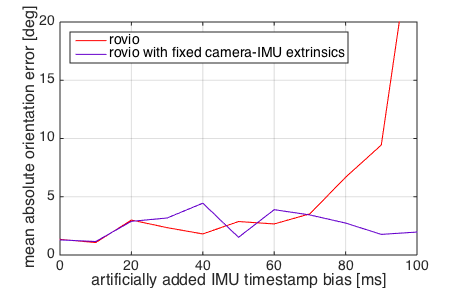
\includegraphics[width=\textwidth]{images/artificial_bias_2.png}
    \caption{}
  \end{subfigure}
   \caption{ROVIO performance on data from the VI-sensor artificially modified by adding a bias between 0 $ms$ and 100 $ms$ on the IMU timestamp: (a) shows the mean absolute translation error, (b) shows the mean absolute orientation error over different timestamp biases. For biases below 50 $ms$, the errors are only slightly increasing. ROVIO diverges on this data with slow dynamics for biases above 90 $ms$. Fixing the extrinsics between camera and IMU helps ROVIO for large timestamp biases.}
   \label{pics:timesync_artificial}
\end{figure}

Figure \ref{pics:timesync_artificial} shows the mean absolute translation error and the mean absolute orientation error of ROVIO for artificial timestamp biases between 0 $ms$ (original mode) and 100 $ms$, in steps of 10 $ms$. The evaluation is performed on the second dataset, introduced in section \ref{sec:euroc}. 

The first observation is that, for this slow dynamic dataset, ROVIO is only diverging with an artificial timestamp bias of 100 $ms$ and stays quite accurate until 50 $ms$. The second observation is, that it is mainly the online estimation of the translational and rotational extrinsics between camera and IMU, which cause the filter to diverge. By fixing these extrinsics and reducing some degrees of freedom within the filter state, ROVIO is even more robust regarding a bias on the IMU timestamp. Fixing the camera-IMU extrinsics can only help if an accurate calibration is available and the extrinsics stay constant during operation since errors within the extrinsics will directly effect the accuracy.



\subsection{ROVIO results with and without time synchronization}
\label{sec:timesync_real}

To test and compare ROVIO on two sensor systems with and without time synchronization, the sensor setup shown in figure \ref{pics:vi_bluefox} has been designed. It consists out of the VI-sensor and an added bluefox 2.0 camera, which has the same characteristics and the same field of view as the camera on the VI-sensor. With this setup, ROVIO running with the hardware-wise time synchronized data of the VI-sensor can be compared with ROVIO running on the hardware-wise non time synchronized data of the bluefox camera and the VI-sensor-IMU. Two datasets with different dynamics have been collected. The first contains slow motions (1.5 $\frac{m}{s}$ and 1 $\frac{rad}{s}$), the second contains fast and shaky dynamics (2.5 $\frac{m}{s}$ and 5 $\frac{rad}{s}$). Ground truth is given by a vicon system. For both datasets the camera was hand-held and facing in direction of movement. A distance of 60 $m$ was collected for each set, which corresponds to three loops within the vicon room. \\

\begin{figure}[h]
   \centering
   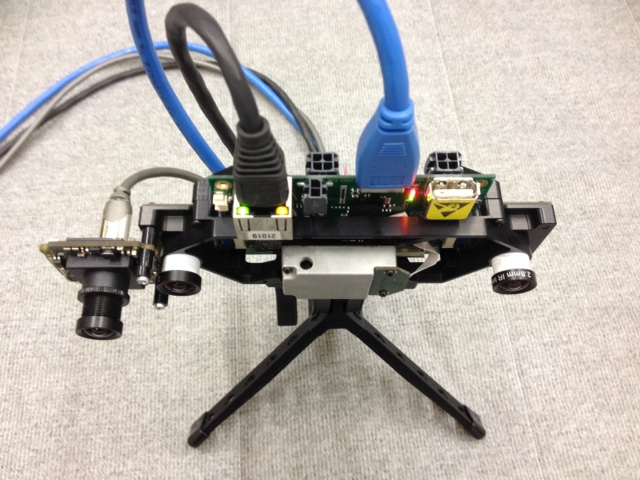
\includegraphics[width=0.4\textwidth]{images/vi_bluefox.JPG}
   \caption{The experimental sensor setup: a bluefox 2.0 camera (left) is added to the VI-sensor. The bluefox camera has the same characteristics and field of view as the camera of the VI-sensor.}
   \label{pics:vi_bluefox}
\end{figure}

For the dataset with slow dynamics (figure \ref{pics:timesync_slow}), ROVIO is principally able to track the motion of the sensor system for both the hardware-wise time synchronized data (VI-sensor) and the non time synchronized data (bluefox and VI-sensor-IMU). Not too surprisingly, the tracking performance of ROVIO running on the VI-sensor data is more accurate (see also appendix \ref{pics:appendix_slow}). The more important result is, that ROVIO, running with the non time synchronized setup, is also able to track these slow motions. \\

\begin{figure}
  \begin{subfigure}[b]{0.46\textwidth}
    \captionsetup{skip=6pt}
    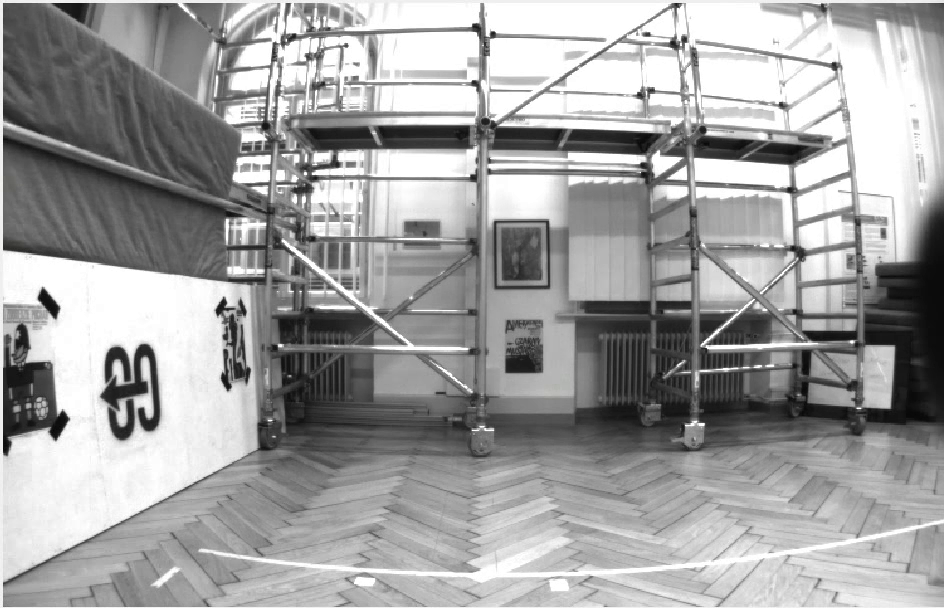
\includegraphics[width=\textwidth]{images/slow.png}
    \caption{}
  \end{subfigure}
  \hfill
  \begin{subfigure}[b]{0.42\textwidth}
    \captionsetup{skip=6pt}
    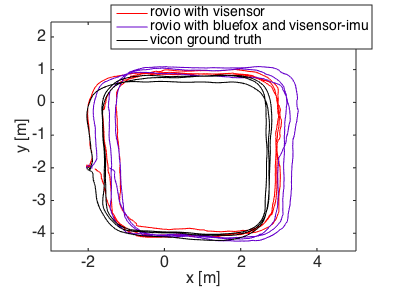
\includegraphics[width=\textwidth]{images/slow_2D.png}
    \caption{}
  \end{subfigure}
   \caption{(a) shows a sample image for the two datasets. Both sets have been collected in a vicon room with lots of visible landmarks. (b) shows the tracking performance of ROVIO on the slow dataset, once with time synchronization (VI-sensor) and once without time synchronization (bluefox and VI-sensor-IMU). ROVIO is principially able to track the motion of the sensor system on both data.}
   \label{pics:timesync_slow}
\end{figure}

For the dataset with fast motions, the outcome is different (figure \ref{pics:timesync_fast} a). ROVIO running with the non time synchronized data is diverging on this set. ROVIO running with the time synchronized data is not diverging; comparing with the slow dataset the errors are significantly increasing (see also appendix \ref{pics:appendix_fast}), but tracking is not lost. If we fix the extrinsics between camera and IMU and hence reduce the number of degrees of freedom in the filter state, ROVIO can be prevented from divergence also on this fast dataset (figure \ref{pics:timesync_fast} b). \\

\begin{figure}
  \begin{subfigure}[b]{0.48\textwidth}
    \captionsetup{skip=6pt}
    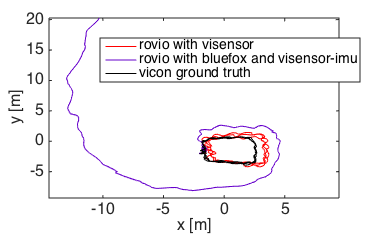
\includegraphics[width=\textwidth]{images/fast_2D.png}
    \caption{online estimated camera-IMU extrinsics}
  \end{subfigure}
  \hfill
  \begin{subfigure}[b]{0.48\textwidth}
    \captionsetup{skip=6pt}
    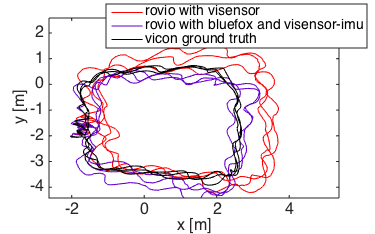
\includegraphics[width=\textwidth]{images/fast_fixed_2D.png}
    \caption{fixed camera-IMU extrinsics}
  \end{subfigure}
   \caption{ROVIO is diverging (a) with the non time synchronized data (bluefox and VI-sensor-IMU) for the dataset with fast and shaky motions, while still able to track with the time synchronized data (VI-sensor). (b) Fixing the extrinsics between camera and IMU on the non time synchronized data prevents the algorithm from divergence.}
   \label{pics:timesync_fast}
\end{figure}

Summarizing the most important results on the analysis towards a non time synchronized sensor setup, we found that

\begin{itemize}
\item ROVIO is principially able to run with a hardware-wise non time synchronized sensor system,
\item the performance of ROVIO with hardware time synchronization is better,
\item hardware time synchronization gets important for high dynamics, and,
\item fixing the extrinsics between camera and IMU can increase the robustness of ROVIO regarding time synchronization.
\end{itemize}

As a future work, these results encourage to go a step further and run ROVIO on an embedded system with a hardware-wise non time synchronized sensor system.













